\documentclass[12pt]{article}
\usepackage[utf8]{inputenc}
\usepackage{cite}
\usepackage{float}
\usepackage{listings}
\usepackage[scale=0.75]{geometry}
\usepackage[hidelinks]{hyperref}
\usepackage{graphicx}
\usepackage{mathtools}
\usepackage{xcolor} % for setting colors
\author{Carlos Bergillos, Antoni Rambla, Adrià Cabeza\\ Departament de Computació}
\title{Document similarity detection using hashing }
\date{\today}
\lstset{
    numbers=none,
    commentstyle=\color{red}, % comment color
	breaklines=true,showstringspaces=false,
  	postbreak=\mbox{\textcolor{red}{$\hookrightarrow$}\space},
	tabsize = 2,
	language=C
}

\begin{document}
  \maketitle  

  \vspace{2cm}
	\begin{abstract}

Our goal is to identify similarities between documents. We have used the Jaccard Similarity theorem,  \textit{Local-Sensitive Hashing} algorithm
 and a \textit{k-shingles} and \textit{minhash signatures} representation of documents to evaluate the effectivity of the similarity computed and the time of computation. We have introduced three different hash functions to see its differences in performance.  Also  once determined the best parameters, we will give a conclusion about the best way to identify the more similar documents. 
\end{abstract}

\newpage
\tableofcontents
\newpage

\section{Introduction}

Our goal is to identify similarities between documents. We say that two documents are similar if they contain a significant number of common substrings that are not too small. 

The problem of computing the similarity between two files has been studied extensively and many programs have been developed to solve it. Algorithms for the problem have numerous applications, including spelling correction systems, file comparison tools or even the study of genetic evolution.

 Existing approaches can also include a brute force approach of comparing all sub-strings of pair of documents. However, such and approach is computationally prohibitive. 

 In our case we have represented each document using a k-shingles set of strings, and implemented algorithms to calculate the Jaccard Similarity and an approximation of it using a \textit{Local-Sensitive Hashing} algorithm
 based on \textit{minhash signatures}.


 
\section{Concept of similarity} \label{similarity}
First we have to focus into the definition of similarity, when we talk about the ``Jaccard similarity'',which is calculated by looking at the relative size of their intersection. 

The Jaccard similarity, also known as Jaccard index is a statistical measure of similarity of sets. For two sets, it is defined as the size of the intersection divided by the size of the union of the sample sets. Mathematically,
\bigbreak
\centerline{\large $J(A,B)=\frac{\left |A\cap B  \right |}{ \left |A\cup B  \right |} = \frac{\left |A\cap B  \right |}{ \left|A\right|+\left|B\right|-\left |A\cap B  \right |} $}
\bigbreak

Calculating the similarity estimation using this approach could be solved using \textit{k} independent repetitions of the MinHash algorithm, however this would require $O(k \times |A|)$ running time. \\\medskip

Let's see an example of how the Jaccard Similarity can be calculated: \\ \\
$A = \{0,1,2,5,6\}$,\\
$B = \{0,2,3,4,5,7,9\}$ \\
$J(A,B) = |A \cap  B| / |A \cup B| = |{0,2,5}| / |{0,1,2,3,4,5,6,7,9}| = 3/9 = 0.33$\\\medskip


The complexity of our implementation is $O(n)$. To calculate the intersection of both sets we use two iterators that iterate through both sets. When an element of a set is smaller than the other we increment its iterator and when they are equal we iterate both and a counter. Finally we use the value of the counter to apply the formula. 

\begin{center}
\begin{large}
Pseudocode Jaccard Similarity
\end{large}
\end{center}

\begin{lstlisting}
Intersection(A,B){
	result = 0; 
	auto it = A.begin(), it2 = B.begin();
	while(it!= A.end() and it2 != B.end()){
		if(*it < *it2){
			++it;
		}
		else if(*it > *it2){
			++it2;
		}
		else {
			++it;
			++it2;
			++result;
		}
	}
	return result; 
}

Jaccard(A, B){
	intersection = intersection(A,B);
	result = intersection / (A.size() + B.size() - intersection);
}

\end{lstlisting}

\textbf{The source code for this section can be found in `\textit{jaccard.cc}'.}
\bigskip

If we take in account the cost of building a set we should observe that for unsorted sequences our cost would be incremented to $O(n \times log(N))$.


%In the case of finding similarities in text a slightly different approach is required. First, it is important to observe that testing whether two documents are exact duplicates is easy; just comparing the two documents characther-by-character would work. However, even if the documents are not identical, they can share large portions of their text.
\section{Representation of documents} \label{Representation}

To identify lexically similar documents we need a proper way to represent documents as sets and the most effective way is to construct from the document the set of short strings that appear within it. If we do so, even if the documents have different sizes or those sentences appear in different order we will find several common elements. In the next section we will introduce some of the approaches of shingling and its variations.

\subsection{\textit{k}-Shingles} \label{kShingles}

A k-shingle (or word-k-gram) is a sequence of consecutive words of size k. Intuitively, two documents A and B are similar if they share enough k-shingles. By performing union and intersection operations between the k-shingles, we can find the Jaccard similarity coefficient between A and B. 
\\
There are some variations regarding on how white space (blank, tab, newline, etc) is treated. Also there is a variation that works with a bag of shingles instead of a set to keep the number of appearances of a shingle. \medskip \\
\\
How large k should be depends on how long typical documents are and how large the set of typical characters is. For example if we pick k = 4 there are $27^4=531441 $ possible k-shingles. However, the calculation can be a little bit more subtle because all the characters do not appear with equal probability. A good rule of thumb is to imagine that there are only 20 characters and estimate the number of k-shingles as $20^k$. For large documents, choice k = 9 is considered safe. 

\subsubsection{Hashing Shingles}

Instead of using substrings directly as shingles, we can pick a hash function that maps strings of length k to some number of buckets and treat the resulting bucket number as the shingle. That process compacts our data and lets us manipulate shingles by single-word machine operations.

\section{MinHash}

A minhash function on sets is based on a permutation of the universal set. Given any such permutation, the minhash value for a set is that element of the set that appears first in the permuted order. 

This algorithm provides us with a fast approximation to the Jaccard Similarity. The concept is to condense the large sets of unique shingles into a much smaller representations called ``signatures''. We will then use these signatures to measure the similarity between document, the signature won't give us the exact similarity but we will get a close estimate (the larger the number of signatures you choose, the more accurate the estimate). In this case we define the similarity like: 
 \medskip

$$  sim(a,b) = \frac{1}{t} \sum_{i=1}^{t}\left\{
1  \; \; \;  if \; \;  a_{i} = b_{i} \\
\; \; \;  or \; \; \;  0 \; \; \;   if\: \;  a_{i} \neq  b_{i} 
\}\right.  $$\medskip


To implement the idea of generating randomly permuted rows, we don't actually generate the random numbers, since it is not feasible to do so for large datasets, e.g. For a million items you will have to generate a million integers..., not to mention you have to do this for each signatures that you wish to generate. One way to avoid having to generate n permuted rows is to pick n hash functions in the form of :
\medbreak
\begin{center}
$ h(x)=(ax+b)\  mod(c)$
\end{center}

Where: 
\begin{itemize}
\item x is the row numbers of your original characteristic matrix
\item a and b are any random numbers smaller or equivalent to the maximum number of x 
\item c is a prime number slightly larger than the total number of shingle sets. 
\end{itemize}

\subsection{Getting the similarity}
To compute the similarity between two documents we only have to traverse the signature matrix once and do an operation similar to the jaccard similarity. The complexity of this algorithm is $O(h)$ where h is the number of hash functions desired.
\begin{center}
\begin{large}
Pseudocode Similarity Between Two Documents
\end{large}
\end{center}
\begin{lstlisting}
sim(signatureMatrix,a,b)
    float simil = 0;
    for i = 0 to signatureMatrix.size() do:
        if(signatureMatrix[i][a] == signatureMatrix[i][b]) then ++simil;
 
    return simil / signatureMatrix.size();


\end{lstlisting}

\textbf{The source code for this section can be found in `\textit{jaccardaprox.cc}'.}
\bigskip

\section{Locality-Sensitive Hashing for Documents}
 This technique allows us to avoid computing the similarity of every pair of sets or their minhash signatures. If we are given signatures for the sets, we may divide them into bands, and only measure the similarity of a pair of sets if they are identical in at least one band. By choosing the size of bands appropriately, we can eliminate from consideration most of the pairs that do not meet our threshold of similarity.
 
 \bigskip
 We define the threshold as the value in which the probability of being taken as a candidate is 1/2, for low thresholds as soon as there is some similitude between documents, we will take them as candidates and vice-versa for high thresholds. An approximation to compute the value of the threshold is as it follows:
 $$Threshold = (1/b)^{1/r}$$
 Where b is the desired number of bands and r is the number of rows (note that $b*r = h$)
 
 \bigskip
If we are looking for speed we want to set the threshold as high as possible so that we find only the documents that look more alike. If what we want is a thorough search, lowering it will allow us to find documents that may only have similar sections.
\medskip 
 
\subsection{Hash function used to hash a vector}
This is the code used to hash a row. It consists on a series of XOR operations on each element of the vector together with a random hexadecimal number and the shifting the value of "seed" from the previous iteration some bits to the left and to the right. The time complexity of this algorithm is $O(n)$ being n the size of the vector. 
\begin{center}
\begin{large}
Pseudocode Vector Hashing
\end{large}
\end{center}
 \begin{lstlisting}
hash_vec(V) {
	seed = V.size();
	for each i in V do:
		seed = seed XOR (i + 0x9e3779b9 + (seed << 6) + (seed >> 2));
		//operands << and >> are shifting left and right respectively x bits
	return seed;
}

\end{lstlisting}

\bigskip
\textbf{Our C++ implementation can be found in function \textit{hash\_vec} in `\textit{\mbox{jaccardaprox.cc}}'}

\subsection{Filling the characteristic matrix} \label{fillingCharacMatrix}
The characteristic matrix is the one we use to represent the shingles that each document has ({see \autoref{Representation}). 

\bigskip
The complexity of the algorithm we use to fill it is $O(n*m)$ where $n$ is number of rows of the matrix (the number of unique k-shingles) and $m$ is the number of columns of the matrix (the number of documents).

\begin{itemize}
\item characMatrix is the characteristic matrix (empty at the beginning of the algorithm)
\item shingles is ordered set containing all the shingles we have in total
\item docShing is a vector of sets in which in position i we have the set of shingles for document i. 
\end{itemize}
 \begin{center}
\begin{large}
Pseudocode To Fill The Characteristic Matrix
\end{large}
\end{center}
 \begin{lstlisting}
fill(characMatrix, shingles, docShing){
    for each row i of characMatrix do:
        for each column j of characMatrix do:
            if docShing[j] contains shingles[i] do:
            	characMatrix[i][j] = 1;
            else
            	characMatrix[i][j] = 0;
\end{lstlisting}

\bigskip
\textbf{Our C++ implementation can be found in function \textit{fill} in `\textit{\mbox{jaccardaprox.cc}}'}

\subsection{Computing the signature matrix} \label{computingSignMatrix}
The signature matrix is the one resulting from finding for each hash function that we have applied and for every document, the first row where there appears a 1 in its permutation.
To compute the signature matrix we use one of the three algorithms.
\begin{itemize}
\item modular hashing
\item multiplicative hashing
\item murmur hashing 
\end{itemize}
The time complexity of this algorithm is tricky as we have to take into account the cost of the hashing algorithm used. Usually the time will be $O(n*m*h*\zeta)$ where $n$ and $m$ are the number of rows and columns of the characteristic matrix respectively, $h$ is the number of hashing algorithms that we use and $\zeta$ is the cost of computing the hash value.
Albeit we use the algorithms only to compute the hash to do row permutations, we follow a general schema to fill it that goes as it follows:

 \begin{center}
\begin{large}
Pseudocode To Compute The Signature Matrix
\end{large}
\end{center}
\begin{lstlisting}
initialize signature matrix with infinity values
for each row i of signatureMatrix do:
	for each column j of signatureMatrix do:
		if(characteristicMatrix[i][j] == 1) then
			for k = 0 to h do:	//h is the number of hash functions that we need
				rowPermutated = value of hash algorithm for row i
				//note that we always use the same algorithm
				if(rowPermutated < signatureMatrix[k][j])
					signatureMatrix[k][j] = rowPermutated;
\end{lstlisting}

\bigskip
\textbf{Our C++ implementations can be found in functions \textit{\mbox{modularHashing}}, \textit{\mbox{multiplicativeHashing}} and \textit{\mbox{murmurHashing}} in `\textit{\mbox{jaccardaprox.cc}}'}

\subsection{LSH and candidate pairs}
As we have mentioned in the beginning of this section, by choosing the size of bands and rows appropriately we augment the number of false positives, documents that have very little in common, or the number of false negatives, documents that have a lot of common but are not checked. 

\bigskip
The time complexity for this algorithm in the worst case (when all the columns of the signature matrix are identical) is $O(b*m*(r+m)) = O(h*m^2)$ where: 
\begin{itemize}
\item m is the number of documents
\item h is the total number of hash functions
\item b is the number of bands
\item r is the number of hash functions per band
\end{itemize}
 \begin{center}
\begin{large}
LSH Pseudocode
\end{large}
\end{center}

\begin{lstlisting}
LSH(signatureMatrix,r,h)
    set<unordered pair<integer,integer>> candidats;                     
    map<integer, set<integer>> bucket;
    for each band i of signatureMatrix do:
        bucket.clear();
        for each column j of signatureMatrix do:
            doc1 = hash_vec of the elements in this band and column
            if (bucket contains doc1 as key) do:
            	for all integers k in bucket[doc1] do:
            		add unordered pair<j, k> to candidats
            	add j to bucket[doc1]
            else
            	bucket[doc1] = new set {j}
            	
    return candidats;

 \end{lstlisting}

\bigskip
\textbf{Our C++ implementation can be found in function \textit{LSH} in `\textit{jaccardaprox.cc}'}
\newline
 
\section{Hashing} \label{hashing}

Hashing is a technique for dimensionality reduction. It uses a hash function that is any function that can be used to map data (called a key) of arbitrary size to data of a fixed size (called a hash value or hash). That hash is a sum up of everything that is in the data. You can never make it backwards from the hash to the data.

Hashing is done for indexing and locating items in databases because it is easier to find the shorter hash value than the longer string.

The hash functions that we want to use need to be: 

\begin{itemize}
\item \textbf{Really fast}\\
Dimensionality reduction is often a time bottle-neck and using a fast basic hash function to implement it may improve running times significantly. 
\item \textbf{Avoid hash collisions}\\
We do not want to get the same hash using different pieces of data %(DIR ALGU DEL pidgeon hole principle)
\item \textbf{Uniform distribution}\\
The hash values are uniformly distributed.
%TODO: mirar, no estic segur de quines característiques necessitem, també he vist altres distribucions, en llop va ficar també que fossin independents

\end{itemize}

In our project we have not chosen hash cryptographic functions (i.e. sha-1 or md5) because they are too slow for our purpose.

\subsection{Modular Hashing}

In the modular hashing (also called the division method), we map a key $k$ into one of $m$ slots by taking the reminder of k divided by m. It takes the following form. 

\begin{center} $h(k) = (ak+b)\  (mod \ m))$ \end{center}

Where: 
\begin{itemize}
\item a and b are any random numbers smaller or equivalent to the maximum number of k 
\end{itemize}

When using the division method, we usually avoid certain values of $m$. For example, $m = 2^p$ for some integer $p$, then $h(k)$ would be just the $p$-lowest-order bits of $k$. A prime value is often a good choice of $m$.

\begin{center}
\begin{large}
Pseudocode Modular Hashing
\end{large}
\end{center}

\begin{lstlisting}[mathescape=true]
ModularHashing(k)
	$x \leftarrow the \ maximum \ value \ possible \ of \ k $
	$a \leftarrow random \ number \ mod\  (x) $
	$b \leftarrow random \ number \ mod\  (x) $
	$m \leftarrow a \ prime \ number \geq x $
	$value \leftarrow a \times k + b \ mod\  (m) $

\end{lstlisting}

\textbf{The source code for this section can be found in `\textit{ModularHash.cc}'.}
\bigskip

\subsection{Multiplicative Hashing}
The multiplicative method for creating hash functions operates in two steps.
Firstly, we multiply the key $k$ by a constant $A$ in the range $0<A<1$ and extract the fractional part of $kA$. Then, we multiply this value by $m$ and take the floor the result. To sum up:  

\begin{center}
 $ \lfloor m\ kA \times mod(1)  \rfloor$
\end{center}
Where:
\begin{itemize}
\item $kA  \times mod(1)$  is the fractional part of $kA$, that is, $kA- \lfloor kA \rfloor$
\end{itemize}
An advantage of the multiplication method is that the value of m is not critical. We typically choose it to be a power of 2 ($m = 2^r$ for some integer $r$), since we can then easily implement the function on most computers.

\vspace{0.4cm}
Supposing that the word size of the machine is $w$ bits, that $k$ fits in a single word and $p$ is the number of bits that you want for the size of your hash value.

 We restrict $A$ to be a fraction of the form, where s is an integer in the range $0<s<2^w$. We first mulitply k by the w-bit integer $s = A\times 2^w$. The result is a $|2 \times w| $-bit value. The desired p-bit hash value consists of the p most significant bits of $r_0$. 


\begin{figure}[H]
	\centering
	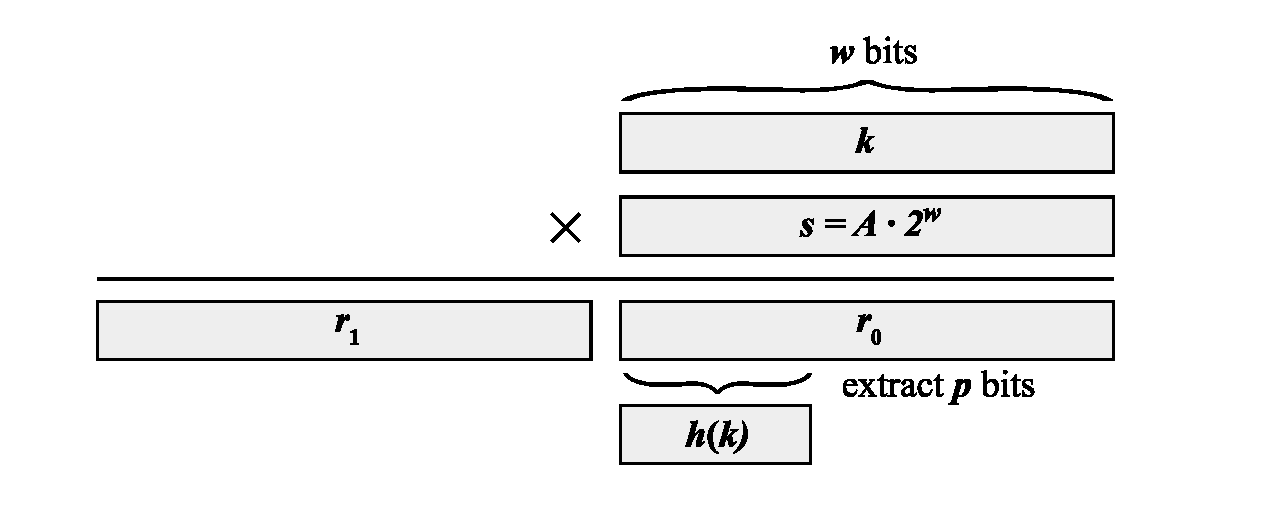
\includegraphics[scale=0.7]{graphs/MultiplicativeHashingDiagram.pdf}
	\caption{Multiplicative Hashing}
	\label{fig:MultiplicativeHashing}
\end{figure}

\bigskip

Although this method works with any value of the constant A, it works better with some values than with others. The optimal choice depends on the characteristics of the data being hashed. Donald Knuth suggest that...

$ A = (\sqrt{5} -1)/2 \simeq 0.6180339887  $

...is likely to work well. So that's why we used this value as an starting point to generate different multiplicative hash functions.
\bigskip

\begin{center}
\begin{large}
Pseudocode Multiplicative Hashing
\end{large}
\end{center}

\begin{lstlisting}[mathescape=true]
MultiplicativeHashing(k,p)

	$A \leftarrow (\sqrt{5} -1)/2 \simeq 0.6180339887 $
	$s \leftarrow A\times 2^w$
	$r \leftarrow k \times s$ 
	$r_0 \leftarrow r\ mod\  (2^w) $ 
	$value \leftarrow r_0 >> (w-p)$

\end{lstlisting}

\textbf{The source code for this section can be found in `\textit{MultiplicativeHash.cc}'.}
\bigskip



\subsection{Murmur Hash}

Consists in applying some multiplications (MU) and rotations (R) to the entry bytes to obtaint the hash. It uses multiple constants which are decided to make it a good hash function by passing 2 basic tests, the Avalanche Test that evaluates how the output changes if the input is slightly modified and the statistical Chi-Squared Test. We have based the implementation of this hash function on Austin Appleby's implementation. Source : \url{https://sites.google.com/site/murmurhash/}\\
\medskip
\begin{center}
\begin{large}
Pseudocode extracted from Wikipedia
\end{large}
\end{center}

\begin{lstlisting}[mathescape=true]
Murmur3(key, len, seed)
    c1 $\leftarrow$ 0xcc9e2d51
    c2 $\leftarrow$ 0x1b873593
    r1 $\leftarrow$ 15
    r2 $\leftarrow$ 13
    m $\leftarrow$ 5
    n $\leftarrow$ 0xe6546b64
 
    hash $\leftarrow$ seed

    for each fourByteChunk of key
        k $\leftarrow$ fourByteChunk

        k $\leftarrow$ k $\times$ c1
        k $\leftarrow$ (k ROL r1)
        k $\leftarrow$ k $\times$ c2

        hash $\leftarrow$ hash XOR k
        hash $\leftarrow$ (hash ROL r2)
        hash $\leftarrow$ hash $\times$ m + n

    with any remainingBytesInKey
        remainingBytes $\leftarrow$ remainingBytes $\times$ c1
        remainingBytes $\leftarrow$ (remainingBytes ROL r1)
        remainingBytes $\leftarrow$ remainingBytes $\times$ c2

        hash $\leftarrow$ hash XOR remainingBytes
 
    hash $\leftarrow$ hash XOR len
    hash $\leftarrow$ hash XOR (hash >> 16)
    hash $\leftarrow$ hash $\times$ 0x85ebca6b
    hash $\leftarrow$ hash XOR (hash >> 13)
    hash $\leftarrow$ hash $\times$ 0xc2b2ae35
    hash $\leftarrow$ hash XOR (hash >> 16)

\end{lstlisting}

\textbf{The source code for this section can be found in `\textit{MurmurHash3.cc}'.}
\bigskip

\section{Data} %canviar el nom de la secció

\subsection{Real-world data}
\begin{itemize}
\item \textbf{Harry Potter and the Sourcerer Stone}: All the text from the first Harry Potter novel.
\item \textbf{The Lord of The Rings: The return of the King}: The entire script from the last Lord of the Rings movie.
\item \textbf{Star Wars: Heir to the Empire}:  An Star Wars novel by Timothy Zahn. 
\item \textbf{50-word lorem ipsum}: The lorem ipsum text is widely used as a place-holder for text so we decided to take 50 words and make our tests based on permutations of it.
\end{itemize}
In our experiments, to compute similarities and approximations we have done several tests with every kind of document, our most successful ones have been with the smallest (lorem ipsum) as we needed some patterns to appear. We can see that in some cases we have iterated with hundreds of documents to achieve that. 

\subsection{Generating the data} \label{generatingData}

To generate the data for our experiments we have used the \textit{random\_ shuffle} function inside the C++ STL which rearranges the elements randomly of a vector. The function swaps the value of each element with that of some other randomly picked element. Its complexity is $O(n)$ with $n$ being  the distance between first and last minus one.\\

The algorithm we implemented to generate our data consists in traversing all the document once to generate a vector of strings containing all the words, then, as many times as permutations we want, we shuffle the vector and write the result in a document. \\

\section{Experiments}
We designed some experiments in order to test our algorithms, and discover how some of their variables affect the outcome.

\subsection{\textit{k}-shingles Size}
\textbf{The source code for this experiment can be found in `\textit{jocProvesJaccard.cc}'.}
\bigskip

We tested different sizes of $k$ for our k-shingles.
For us, $k$ defines the number of characters for each k-shingle.

Using the algorithm explained in \autoref{generatingData}, we generated 20 permutations of a 50 words document, thus obtaining 20 new documents.

Then we calculated the Jaccard Similarity (section \autoref{similarity}) for all the possible pairs of documents from this set.

The number of possible pair combinations for a set of $n$ elements (where order is not important) is given by $\binom{n}{2}$.

In our case, with a set of 20 documents we have:
\bigbreak
\centerline{\large $\binom{20}{2} = 190$}
\bigbreak

So we computed the Jaccard Similarity for these 190 pairs of documents, for different sizes of $k$, ranging from 2 to 20. The results can be seen in \autoref{fig:KShinglesSimilarity}.

\bigbreak
As we expected, the similarity decreases as the size of the k-shingles increases.

For smaller values of $k$ that allow k-shingles to remain within a word, we see that a lot of similarities are found, as the documents share the same words.
On the other hand, for values of $k$ that span more than one word, the similarity between documents is very small (because the documents don't share the word order, so the probability of identical k-shingles decreases).
In fact, we observe that for values of $k$ larger 12, the similarity obtained is mostly 0.

As mentioned in \autoref{kShingles}, a good and reasonable value for $k$ is 9.
For $k = 9$, the similarity found between all our random documents is less than 0.1, which corresponds with the fact that the documents don't really share sentences or many contiguous words.

\begin{figure}[H]
	\centering
	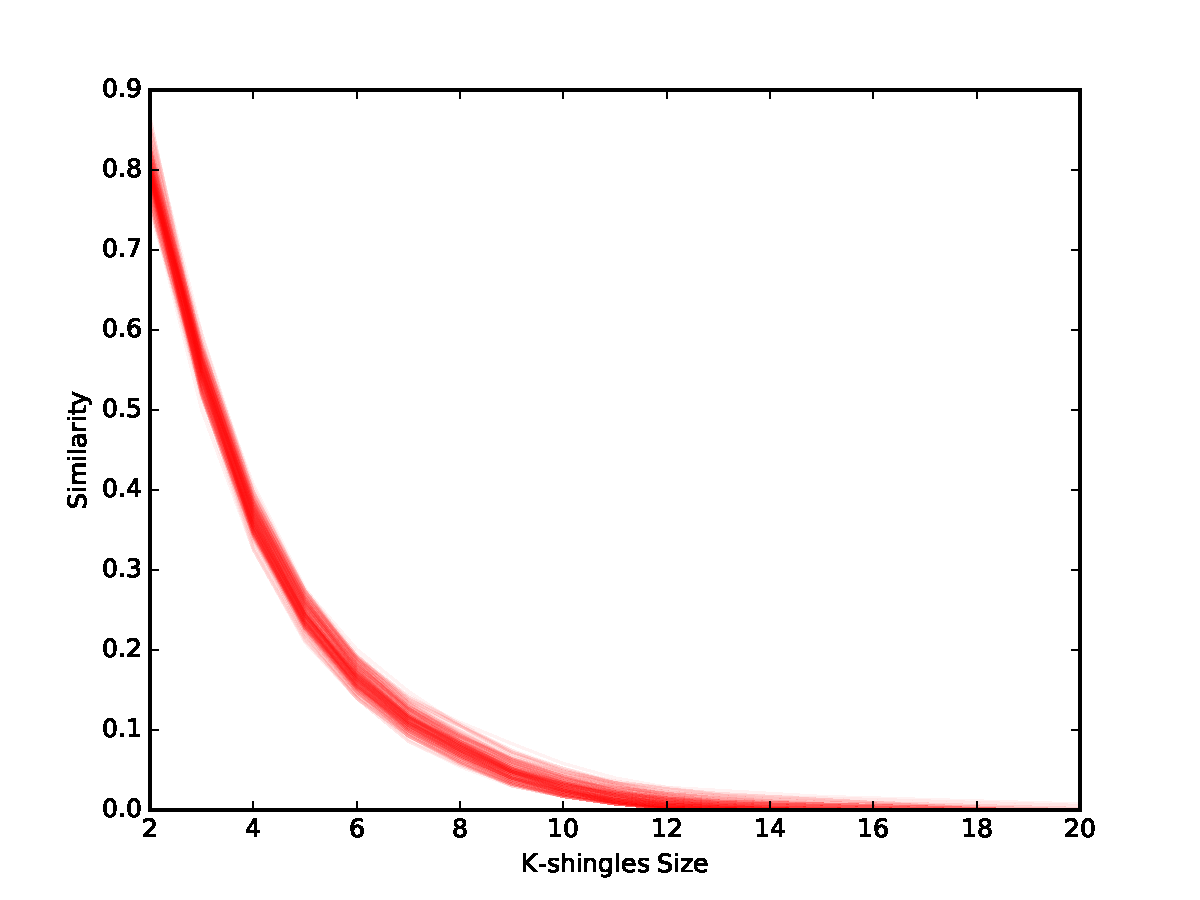
\includegraphics[scale=0.5]{graphs/JaccardSimilarityValueKshingles.pdf} 
	\caption{Relation between the K-shingles size and the similarity (for all of the possible pairwise combinations of 20 random permutations of a 50 words document)}
	\label{fig:KShinglesSimilarity}
\end{figure}

\subsection{Performance of Different Hashing Algorithms}
\textbf{The source code for this experiment can be found in `\textit{jocProvesHashTimes.cc}'.}
\bigskip

We have tested different k sizes for our k-shingles and three different hash functions in the process of filling the signature matrix to check their different performance. The process of filling the signature matrix is explained in the \autoref{computingSignMatrix} and our hash functions are MurmurHash3, Multiplicative Hash and Modular Hash and can be seen more deeply in \autoref{hashing}.

As we expected initially, the time increases as the size of the k-shingle increases. This behavior can be explained using the fact that the number of different shingles we would have to work with would be bigger. It is trivial to observe that the number of different k-shingles is going to have a growing tendency based on their size. 

Also we have been able to observe that the performance of MurmurHash and MultiplicativeHash are almost the same and ModularHash is the one that has performed the best, performing almost always with values smaller than the half of the others two.



\begin{figure}[H]
	\centering
	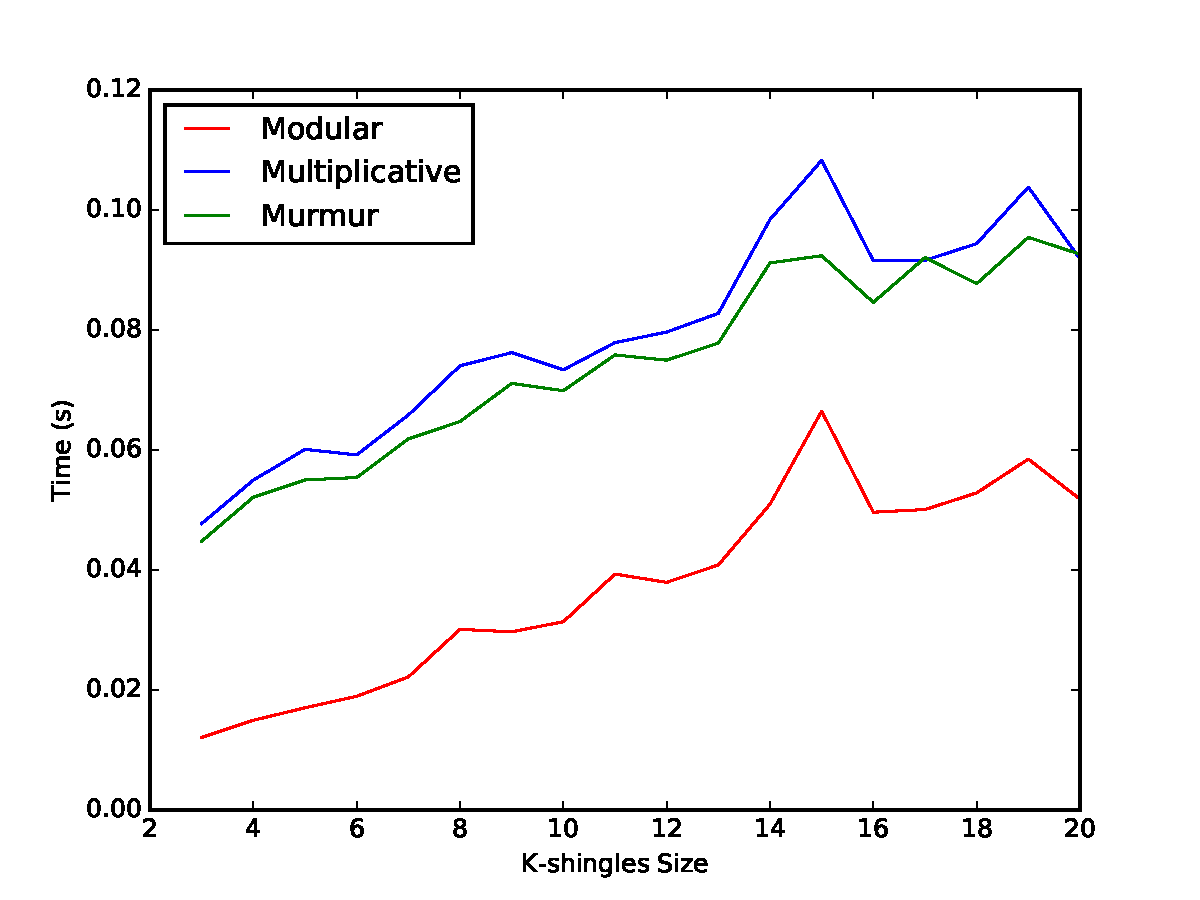
\includegraphics[scale=0.55]{graphs/HashFunctionsJaccardAproxTime.pdf} 
	\caption{Difference between the time used by different Hashing Functions}
	\label{fig:HhashFunctionsTime}
\end{figure}

%\begin{figure}[h]
%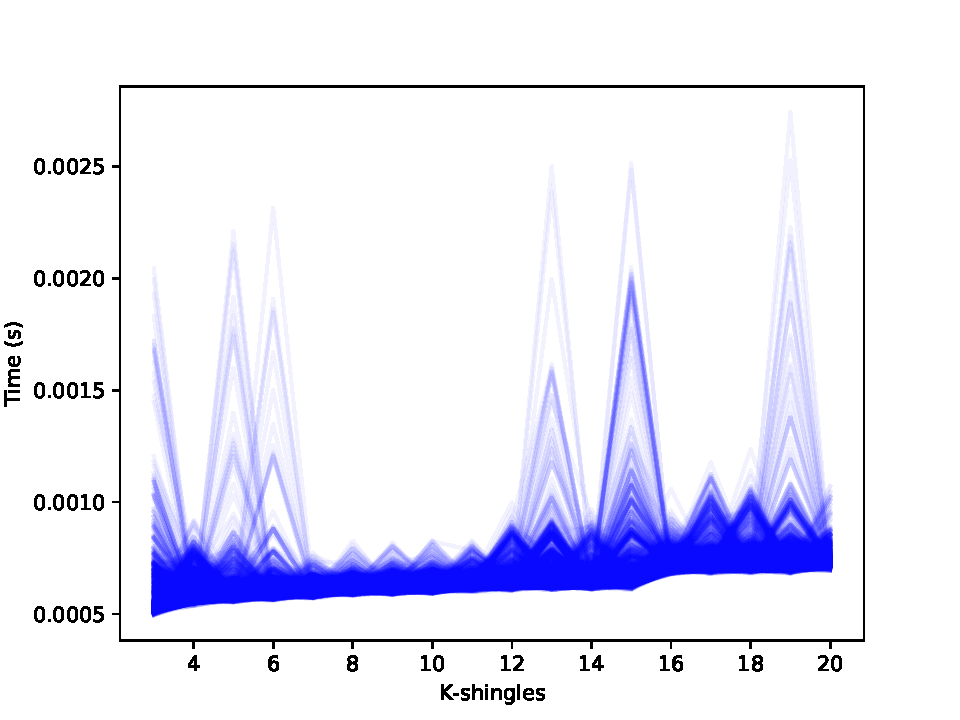
\includegraphics[scale=1]{JaccardSimilarityTimeKshingles.pdf}
%  \caption{Relation between the k-shingles and the time of execution}
%  \label{fig:KShinglesTime}
%\end{figure}

\subsection{Performance of Different Document Similarity Approaches}
\textbf{The source code for this experiment can be found in `\textit{jocProvesJaccSim.cc}'.}
\bigskip

We tested three different approaches to find similarities in a set of documents.
\begin{itemize}
\item Calculating the Jaccard similarity for all the possible pair combinations in the document set.
\item Calculating a Jaccard similarity approximation via a computed signature matrix.
\item Calculating a Jaccard similarity approximation via a computed signature matrix with a locality-sensitive algorithm.
\end{itemize}

Each approach is supposed to perform respectively faster.

\bigskip
We created a set of 410 documents (result of random permutations of a 50-words document, as explained in \autoref{generatingData}). 

We then independently applied these 3 approaches to subsets of gradually increasing size, ending with the whole set of 410 documents, while recording the times of each process.
The plotted results can be found in \autoref{fig:JaccSignLSH}.

All the tests in this experiment were done with k-shingles of size 5, and for the second and third approach, we used 200 hashing functions (resulting in a signature matrix of 200 rows). Additionally, the third approach divided the 200 rows in 20 bands of 10 rows. These parameters were chosen to simulate a plausible real application.

\bigskip

We can observe that the first approach, while being the only one that computes the real Jaccard similarity (and not an approximation), is exponential in nature, and thus, is not feasible for large document sets. In fact, while doing this test, we had to limit the execution of this approach to only sets with less than 100 documents, as it becomes unmanageable otherwise.

The other two approaches are way better alternatives, as they are asymptotically faster.
And, while they seem to both be asymptotically linear, we don't think that's the case.
We don't have the time or computing power to do tests with larger datasets, but the way the second approach is constructed, it iterates through all the $\binom{n}{2}$ possible pairs of documents, which has cost $O(n^2)$, with $n$ being the number of documents.

We believe that most of the computation time is spent constructing the k-shingles set, and constructing the signature matrix, which has a cost of $O(n)$ (see \autoref{fillingCharacMatrix} and \autoref{computingSignMatrix}), and that the similarity calculation for all the possible document pairs represents only a small fraction of the total time for relatively small datasets, thus making it seem of linear behavior.

At the same time, the third approach is also faster than the second one, we can see in \autoref{fig:JaccSignLSH} how they diverge as the size of the datasets increases.
In this case, we believe the cost is still quadratic, but with a way smaller scaling factor, as only a small fraction of the possible $\binom{n}{2}$ document pairs are selected as candidates for similarity checking.
\bigskip

\begin{figure}[H]
	\centering
	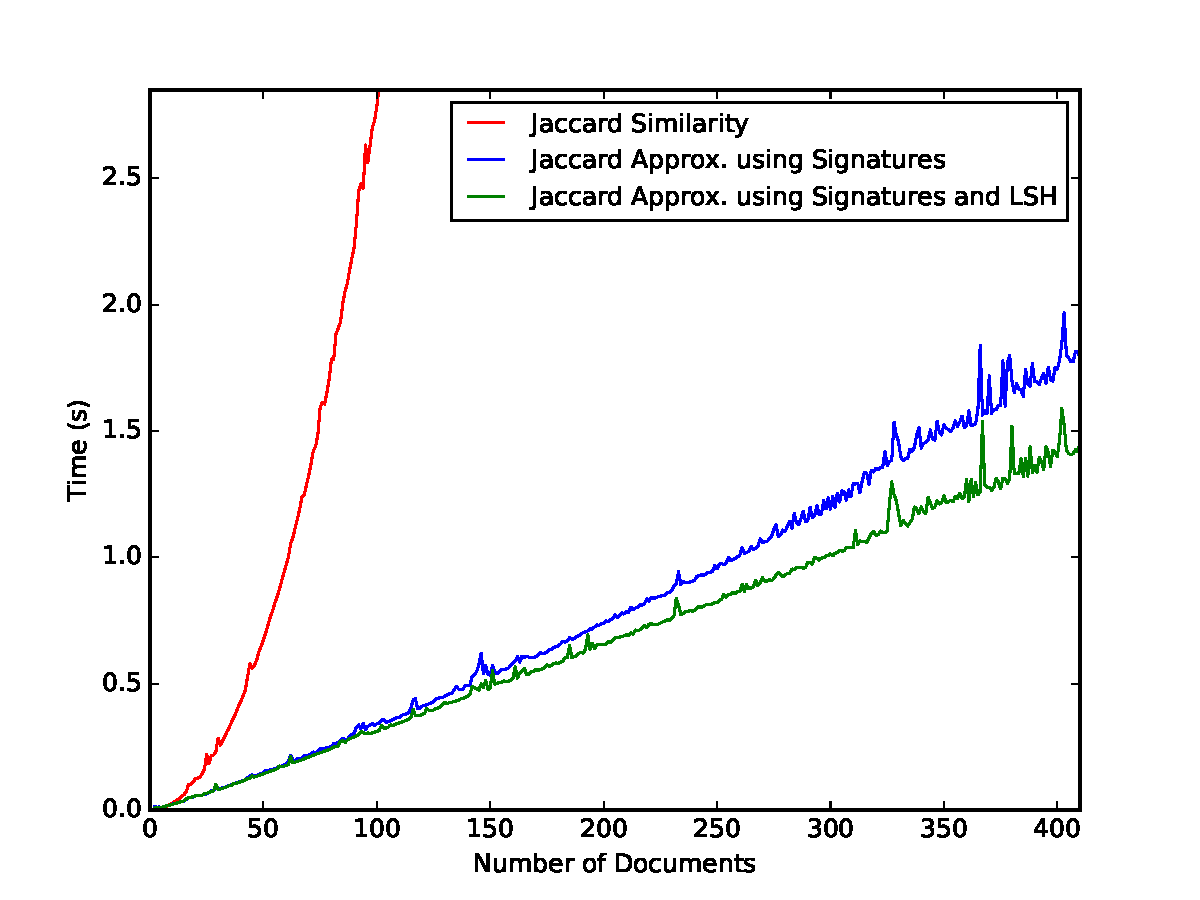
\includegraphics[scale=0.55]{graphs/JaccardSignatureLSHTimes.pdf}
	\caption{Time spent by the three approaches for different sets of documents of increasing size}
	\label{fig:JaccSignLSH}
\end{figure}

\subsection{Precision of Jaccard Similarity Approximations}
\textbf{The source code for this experiment can be found in `\textit{jocProvesJaccSimLsh.cc}'.}
\medskip

In the following experiment we wanted to test how precise the outputed similarity for the MinHash method is. 

\bigskip
In the experiment we have observed how the similarity changes depending on the number of hash functions used. Also we have plotted the Jaccard Similarity value in order to see which is the real similarity for the pair of documents analysed and check how the precision changes. 
All the tests in this experiment were done with a pair of documents with 60\% similarity and with k-shingles of size 9, which is a good value for $k$ as we argued in \autoref{kShingles}. 

\bigskip
As we expected when the number of hash functions is small the difference between the real similarity and the approximation differs a lot. Moreover, as the number of hash functions increases the difference of similarity decreases significantly.  The reason we believe this happens is because albeit the hash functions are not perfect and create collisions, the number of ``good'' permutations outnumbers the ones that collide. Having more functions means that overall we have more ``good'' permutations and thus the impact that the ``bad'' ones have is less significant.


\begin{figure}[H]
	\centering
	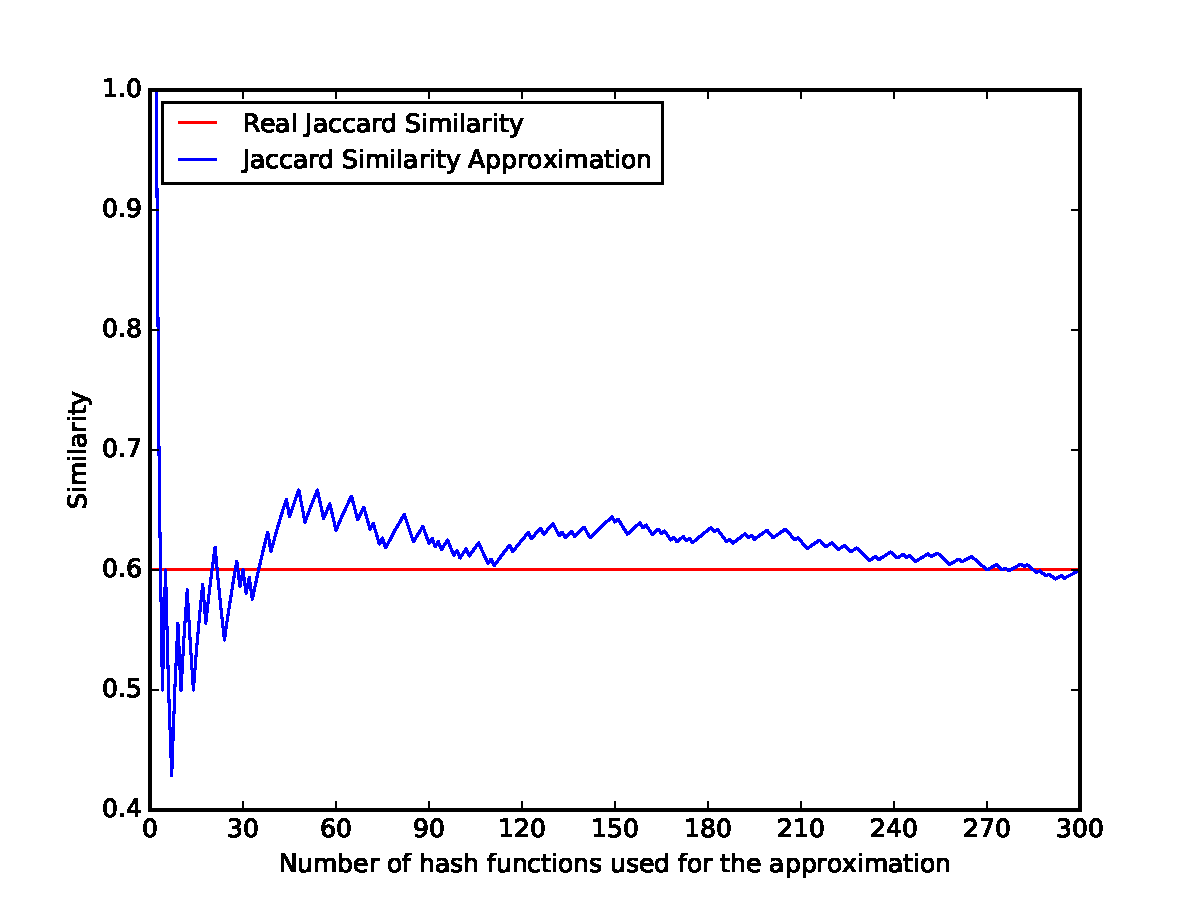
\includegraphics[scale=0.55]{graphs/JaccardSimilarityVsApproximation.pdf}
	\caption{Approximated Jaccard Similarity for a pair of 2 documents with 60\% real similarity (K-shingles size = 9)}
	\label{fig:JaccardVsApprox}
\end{figure}
\subsection{Visualizing the data}
To make it easier for us to compute and visualize graphically the results we have set up a python script which uses the matplot library. Although to generate the aforementioned information first we have to execute the corresponding programs (see the manual) and then the information gets saved in a csv format. When we execute the script we are prompted with a series of options to choose from, obviously if we have not done the experiment chosen beforehand we wont have any data to read and thus we wont have a graphic or we will get a graphic made from previous data.
\clearpage
\section{Conclusions}

\begin{enumerate}
\item Small sizes for k-shingles result in many false positives. And very large sizes for the k-shingles result in very few (if any) similarities being found. 9 can be a good value for general text documents.
\item Larger sizes for the k-shingles result in longer computation times.
\item Of the hashing functions we evaluated, Modular Hashing is the one that performed the best. Resulting in significantly faster computation times than Multiplicative Hashing and Murmur Hashing.
\item Trying to find pairs of similar documents by computing the Jaccard similarity for all the possible pairs is not feasible for large document sets. Jaccard approximation algorithms using minhash signatures produce a very similar result to the real Jaccard similarity, but with a fraction of the cost. And for very large documents sets, locality-sensitive hashing should be considered.
\item Larger number of hash functions result in a better precision for the MinHash method.
\item The bigger the number of documents to compare is, the more important is to use a LSH with the signature matrix as it will have a big impact on the required time.
\item Choosing b and r carefully is important as it means that we can either get several documents which are very dissimilar together or we never band two documents that look the same. It is needed to think beforehand and choose an appropriate value. 
\item It is important to explore different approaches and algorithms to improve either time or the quality of the solution, as we have seen if we only took the Jaccard similarity to compute how similar several documents are we would have gotten an exponential time. After taking the signature matrix (which already highly improves the speed) we use the LSH technique to further improve it.

\end{enumerate}

%http://ethen8181.github.io/machine-learning/clustering_old/text_similarity/text_similarity.html

%mirar aquest algoritme: http://www.xmailserver.org/diff2.pdf
\clearpage
\begin{thebibliography}{100}

\bibitem{Concept of similarity}
J.\ Bank and B.\ Cole,
\textit {Calculating the Jaccard similarity coefficient with map reduce for entity pairs in
Wikipedia} (Wikipedia Similarity Team, 2008).

\bibitem{Mining of Massive Datasets}
J.\ Leskovec, A.\ Rajaraman and J.\ Ullman
\textit{ Finding Similar Items. In Mining of Massive Datasets} (Cambridge University Press, 2014).

\bibitem{O(ND) Difference Algorithm}
E.\ W. Myers \textit{An O(ND) Difference Algorithm and Its Variations} (Department of Computer Science, University of Arizona)

\bibitem{Plagiarism Detection}
S.\ Alzahrani and N. \ Salim, \textit{Fuzzy Semantic-Based String Similarity for Extrinsic Plagiarism Detection} (Taif University, Saudi Arabia and Universiti Teknologi Malaysia, Malaysia)

\bibitem{Hash Functions}
S.\ Dahlgaard, M.\ Tejs Knudsen and M.\ Thorup, \textit{Practical Hash Functions for Similarity Estimation and Dimensionality Reduction} (University of Copenhagen)

\bibitem{Universal string hashing}
D.\ Lemire and O.\ Kaser, \textit{Strongly universal string hashing is fast} (Université du Québec Canadá and University of New Brunswick, Canada) 

\bibitem{C++ STL}
C++ Standard Template Library,
\ Source: \url{cplusplus.com/reference/stl/}




\bibitem{MurmurHash, Wikipedia}
\textit{MurmurHash}. \ Source: \url{https://en.wikipedia.org/wiki/MurmurHash}

\bibitem{MurmurHash, Github}
\textit{MurmurHash alternative source}. \ Source: \url{https://github.com/aappleby/smhasher/wiki/MurmurHash3}

\bibitem{Hash function}
\textit{Hash function}. \ Source: \url{https://en.wikipedia.org/wiki/Hash_function}

\bibitem{Introduction to Algorithms}
T.\ H.\ Cormen, C.\ E.\ Leierson, R.\ L.\ Rivest and C.\ Stein, \textit{Introduction to Algorithms. Third Edition}

\bibitem{Sorting and searching}
D.\ Knuth,
\textit {Sorting and Searching}, volume 3 of \textit{The Art of Computer Programming} (Addison-Wesley, 1997. Third Edition)


\bibitem{Murmur Hash explained}
S.\ Yar [Developer's Catalog By Sahib Yar]
\textit {Sorting and Searching}, \textit{Murmur Hash - Explained} (Youtube, Jun 23, 2017), Retrieved from: \url{https://www.youtube.com/watch?v=b8HzEZt0RCQ&t=1s}

\bibitem{Hashing Algorithms}
T.\ Scoot [Computerphile]
\textit {Hashing Algorithms and Security - Computerphile}, (Youtube, Nov 8, 2013), Retrieved from: \url{https://www.youtube.com/watch?v=b4b8ktEV4Bg&t=181s}

\bibitem{Latex}
L.\ Lamport, \textit{LATEX: a document preparation system: user's guide and reference manual} (Addison-Wesley Pub. Co., cop. 1994)


\end{thebibliography}

\end{document}



\end{thebibliography}

\end{document}

